%!TEX root = ../rsra.tex

\chapter{Availability and Maintainability}
\section{Introduction}
\emph{Can I repair the system after a failure?} We can classify systems into two
categories according to the answer to this question.
\begin{itemize}
    \item \textbf{Non maintained systems} These systems cannot be repaired after a
    failure (e.g. a  telecommunication satellite, a F1 engine, a vessel of a nuclear
    power plant).
    
    $\to$ a good \emph{performance parameter} is the \emph{reliability}, as it
    quantifies the system capability of satisfying a specified mission within an
    assigned period of time ($T_M$): $R(T_M) = P(T>T_M)$

    \item \textbf{Maintained systems} These systems can be repaired after the failure
    (e.g. pump of an energy production plant, a component of the reactor emergency
    cooling systems).
    
    $\to$ a good \emph{performance parameter} is the \emph{availability}, as it
    quantifies the system ability to fulfill the assigned mission at any specific
    moment in the lifetime: $A(t)$.
\end{itemize}

We will now try to give now a more rigorous definition of \emph{availability}.

\section{Definition of Availability}
Let's tackle the problem from a mathematical point of view.

We introduce an indicator variable $X(t)$ such that:
\begin{equation*}
    X(t)=\begin{cases}
        1 & \text{system is operating at time } t \\
        0 & \text{system is failed at time } t
    \end{cases}
\end{equation*}

\begin{figure}[!htp]
    \centering
    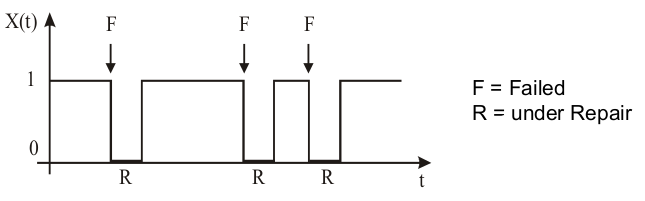
\includegraphics[width=.85\textwidth]{x(t)_example}
    \caption{An example of $X(t)$ for a given system}
\end{figure}

\subsection{Instantaneous availability}
\begin{equation*}
    p(t) = P\{X(t)=1\} = E[X(t)]
\end{equation*}

Notice that:
\begin{equation*}
    E[X(t)] = \sum_{i=0}^1 iP\{X(t)=i\} = 0\cdot P\{X(t)=0\} + 1\cdot P\{X(t)=1\} = p(t)
\end{equation*}

\subsection{Instantaneous unavailability}
\begin{equation*}
    q(t) = P\{X(t) = 0\} = 1 - p(t)
\end{equation*}
where the last equivalence comes from the fact that the two events "system is
operating at time t" and "system is failed at time t" are mutually exclusive.

\section{Contributions to Unavailability}
\subsection{Repair}
A component can be unavailable because it is under repair after a failure.
\begin{figure}[!htp]
    \centering
    
\includegraphics[width=.3\textwidth]{repair}
    \caption{A component could be under repair}
\end{figure}

\subsection{Testing / Preventive Maintenance}
A component can be removed from the system because
\begin{enumerate}[label=\alph*]
    \item it must undergo preventive maintenance (e.g. periodic replacement of a
    transmission belt in a car, see Fig.~\ref{fig:transmission_belt})
    \begin{figure}[H]
        \centering
        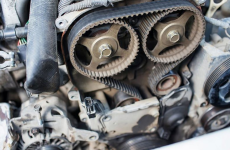
\includegraphics[width=.4\textwidth]{transmission_belt}
        \caption{Transmission belt in a car}
        \label{fig:transmission_belt}
    \end{figure}
    \item it has to be tested, i.e. safety systems and standby components are
    designed to operate only in extremely rare cases and spends most of their
    time in standby, thus requiring proper testing to ensure that they're still
    in good working conditions.
    \begin{figure}[H]
        \centering
        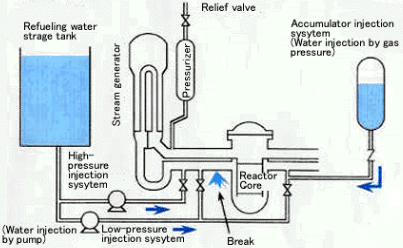
\includegraphics[width=.4\textwidth]{eccs}
        \caption{Emergency Core Cooling System in a Nuclear Power Plant}
    \end{figure}
\end{enumerate}


\subsection{Unrevealed failure}
A stand-by component can fail unnoticed. The system goes on without noticing the
component failure until a test on the component is made or the component is
demanded to function.

\section{Average availability descriptors}
\emph{How to compare different maintenance strategies?} We need to define
quantities for an \emph{average} description of the system probabilistic
behavior:
\begin{itemize}
    \item If after some initial transient effects, the instantaneous
    availability assumes a time independent value $\to$ Limiting or \emph{steady
    state availability}:
    \begin{equation*}
        p = \lim_{t\to \infty} p(t)
    \end{equation*}
    \begin{figure}[H]
        \centering
        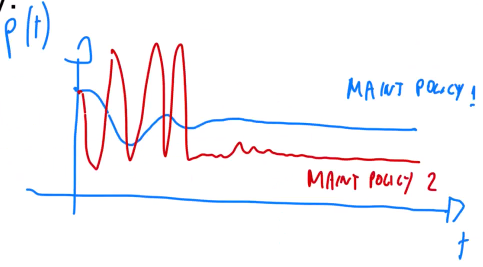
\includegraphics[width=.6\textwidth]{maintenance_policies}
        \caption{Using this descriptor, maintenance policy 2 is \emph{better}}
    \end{figure}
    \item If the limit does not exist (e.g. periodic behavior) $\to$
    \emph{Average availability} over a period of time $T_p$:
    \begin{equation*}
        p_{T_p} = \frac{1}{T_p} \int_0^{T_p} p(t)dt = \dots = \frac{\overline{\mathrm{UPTIME}}}{T_p}
    \end{equation*}
    \begin{equation*}
        q_{T_p} = \frac{1}{T_p} \int_0^{T_p} q(t)dt = \dots = \frac{\overline{\mathrm{DOWNTIME}}}{T_p}
    \end{equation*}
    \begin{figure}[H]
        \centering
        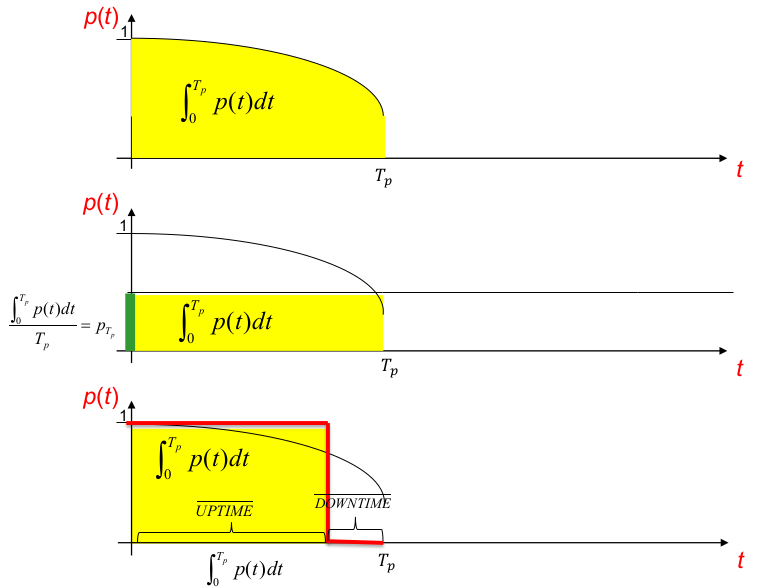
\includegraphics[width=.8\textwidth]{instantaneous_availability}
        \caption{Two equivalent representation of the instantaneous availability that make use of the average availability}
    \end{figure}
\end{itemize}

\section{Maintainability}
\emph{How fast a system can be repaired after failure?} Repair time $T_R$
depends from many factors as seen in Fig.~\ref{fig:repair_time_factors}
\begin{figure}[!htp]
    \centering
    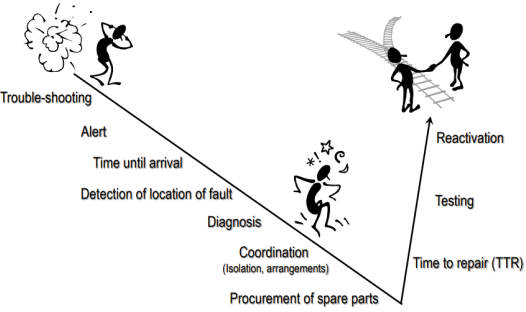
\includegraphics[width=0.6\textwidth]{repair_time_factors}
    \caption{Factors that affect repair time}
    \label{fig:repair_time_factors}
\end{figure}

Repair time $T_R$ varies statistically from one failure to another, depending on
the conditions associated to the particular maintenance events.

Let $T_R$ denotes the downtime random variable, distributed according to the pdf
$g_{T_R}(t)$.

\emph{Maintainability} is defined as the cumulative distribution function:
\begin{equation*}
    P(T_R \le t) = \int_0^t g_{T_R}(\tau)d\tau
\end{equation*}

\section{Failure classification}
\paragraph*{Revealed failure} A failure that may be immediately or almost
immediately apparent through an alarm or indicator system.

\paragraph*{Unrevealed failure} A stand-by component can fail unnoticed. The
system goes on without noticing the component failure until a test on the
component is made or the component is demanded to function.

\section{Revealed failure}
\subsection{Availability of a continuously monitored component}
\subsubsection*{Hypothesis}
\begin{itemize}
    \item Constant failure rate $\lambda$;
    \item Restoration starts immediately after the component failure;
    \item Probability density function of the random time duration $T_R$ of the
    repair process = $g_{T_R}(t)$.
\end{itemize}

\subsubsection*{Objective}
Computation of the availability $p(t)$ of a continuously monitored component.

\subsubsection*{Method}
It is based on a conceptual experiment with $N_0$ identical components that
start at time $t=0$. We then write a balance equation for the number $N(t)$ of
components working between time $t$ and $t+\Delta t$.

%TODO linea temporale

The number of systems working at time $t+\Delta t$ is
\begin{equation*}
    N(t+\Delta t) = N(t) - N_F + N_R
\end{equation*}
where
\begin{itemize}
    \item $N_F$ is the number of systems that fail between $t+\Delta t$
    \item $N_R$ is the number of systems that are repaired between $t+\Delta t$
\end{itemize}

Let's reason in terms of expected value:
\begin{equation*}
    E[N(t+\Delta t)] = E[N(t)] - E[N_F] + E[N_R]
\end{equation*}

\begin{equation*}
    E[N(t+\Delta t)] = N_0\cdot p(t+\Delta t)
\end{equation*}

\begin{equation*}
    E[N(t)]=N_0\cdot p(t)
\end{equation*}

\begin{equation*}
    \begin{split}
        E[N_F] &= N_0\cdot P\{\text{failure between $t$ and $t+\Delta t$}\} \\
        &= N_0\cdot P\{\text{up at time t}\}\cdot P\{\text{failure in }(t;t+\Delta t)|\text{up at time t}\}  \\
        &= N_0\cdot p(t)\cdot \lambda \Delta t
    \end{split}
\end{equation*}

\begin{figure}[!htp]
    \centering
    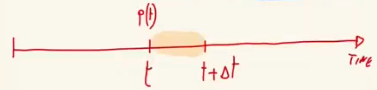
\includegraphics[width=0.6\textwidth]{cont_mon_1}
    \caption{Timeline}
\end{figure}

\begin{equation*}
    E[N_R] = \int_0^t N_0 \cdot p(\tau) \cdot \lambda d\tau \cdot g_{T_R}(t-\tau)\Delta t
\end{equation*}

\begin{figure}[!htp]
    \centering
    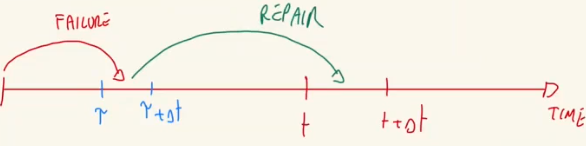
\includegraphics[width=0.6\textwidth]{cont_mon_2}
    \caption{Timeline}
\end{figure}

\begin{equation*}
    N_0p(t+\Delta t) = N_0 p(t) - N_0p(t)\lambda\Delta t + \int_0^t N_0 \cdot p(\tau) \cdot \lambda d\tau \cdot g_{T_R}(t-\tau)\Delta t
\end{equation*}

Dividing both sides by $N_0$,
\begin{equation*}
    p(t+\Delta t) = p(t) - p(t)\lambda\Delta t + \int_0^t \cdot p(\tau) \cdot \lambda d\tau \cdot g_{T_R}(t-\tau)\Delta t
\end{equation*}

\begin{equation*}
    \frac{p(t+\Delta t) - p(t)}{\Delta t} = - p(t)\lambda + \int_0^t p(\tau) \cdot \lambda d\tau \cdot g_{T_R}(t-\tau)
\end{equation*}

The integral-differential form of the balance:
\begin{equation*}
    \lim_{\Delta t \to 0} \frac{p(t+\Delta t) - p(t)}{\Delta t} = \frac{dp(t)}{dt} = - p(t)\lambda + \int_0^t p(\tau) \cdot \lambda d\tau \cdot g_{T_R}(t-\tau)    
\end{equation*}
with $p(0) = 1$

The solution can be obtained introducing the Laplace transforms in Table~\ref{tab:laplace_transforms}.
\begin{table}[!htp]
    \centering
    \begin{tabular}{ll}
        \toprule
        Time domain & Laplace domain \\
        \midrule
        $p(t)$ & $\mathcal{L}[p(t)] = \int_0^{+\infty} e^{-st}p(t)dt = \tilde{p}(s)$ \\[2ex]
        $\frac{dp(t)}{dt}$ & $\mathcal{L}\left[\frac{dp(t)}{dt}\right] = s\cdot \tilde{p}(s) - p(0)$ \\[2ex]
        $p(t)* g(t) = \int_0^t p(\tau)g(t-\tau)d\tau$ & $\mathcal{L}[p(t)* g(t)] = \tilde{p}(s)\cdot \tilde{g}(s)$ \\
        \bottomrule
    \end{tabular}
    \caption{Laplace transforms}
    \label{tab:laplace_transforms}
\end{table}

Applying the Laplace transform we obtain:
\begin{equation*}
    s\cdot \tilde{p}(s) - 1 = -\lambda\cdot \tilde{p}(s) + \lambda\cdot\tilde{p}(s)\cdot\tilde{g}(s)
\end{equation*}
which yields:
\begin{equation*}
    \tilde{p}(s) = \frac{1}{s+\lambda\cdot(1-\tilde{g}(s))}
\end{equation*}

Applying the inverse Laplace transform to $\tilde{p}(s)$, the instantaneous
availability $p(t)$ is determined.

Furthermore, to determine the limiting availability $p_\infty$, the final value
theorem can be exploited:
\begin{equation*}
    p_\infty = \lim_{t\to\infty}p(t) = \lim_{s\to 0} [s\cdot\tilde{p}(s)] = \lim_{s\to 0}\left[\frac{s}{s+\lambda\cdot(1-\tilde{g}(s))}\right]
\end{equation*}

As $s$ tends to 0, a first order approximation of $\tilde{g}(s)$ can be
considered:
\begin{equation*}
    \begin{split}
        \tilde{g}(s) &= \int_0^\infty e^{-s\tau} g(t) d\tau \\
        &= \int_0^\infty (1-s\tau + \dots)g(\tau)d\tau \\
        &\cong 1-s\cdot\int_0^\infty \tau g(\tau)d\tau = 1-s\cdot\text{MTTR}
    \end{split}
\end{equation*}
where the mean-time-to-repair is $\text{MTTR} = \overline{\tau_R} = E_G[T_R]$,
that is to say the expected value of the restoration time distribution $G(t)$.

Hence,
\begin{equation*}
    \begin{split}
        p_\infty &= \lim_{s\to 0} \frac{s}{s+\lambda s \overline{\tau_R}} \\
        &= \frac{1}{1+\lambda\overline{\tau_R}} = \frac{1/\lambda}{1/\lambda+\overline{\tau_R}} \\
        &= \frac{MTTF}{MTTF+MTTR} \\
        &= \frac{\text{average time the component is UP}}{\text{average period of a failure/repair "cycle"}}
    \end{split}
\end{equation*}

%TODO put this line in a box!
\textbf{This result is valid for any repair process $G(t)$!}

\subsection{Example 6.1 (Red Book)}
Find the instantaneous and the limiting availabilites for a component whose
restoration probability density is:
\begin{equation*}
    g(t) = \mu \cdot e^{-\mu\cdot t}
\end{equation*}

\subsubsection*{Solution}
The limiting availability is:
\begin{equation*}
    p_\infty = \lim_{t\to\infty}p(t) = \frac{MTTF}{MTTF+MTTR} = \frac{1/\lambda}{1/\lambda + 1/\mu}
\end{equation*}

\begin{equation*}
    \begin{split}
        \tilde{g}(s) &= \int_0^\infty e^{-s\tau} g(t) d\tau \\
        &= \mu\int_0^{+\infty}e^{-(s+\mu)\tau}d\tau\\
        &= \frac{\mu}{s+\mu}
    \end{split}
\end{equation*}

\begin{equation*}
    \begin{split}
        \tilde{p}(s) &= \frac{1}{s+\lambda\cdot(1-\tilde{g}(s))}\\
        &= \frac{1}{s+\lambda\cdot\frac{s}{s+\mu}} = \frac{s+\mu}{s^2+\mu s+\lambda s}
    \end{split}
\end{equation*}

\begin{equation*}
    p(t) = \mathcal{L}^{-1}\left[\frac{s+\mu}{s^2+\mu s+\lambda s}\right]
\end{equation*}

\begin{equation*}
    \tilde{p}(s)= \frac{A}{s} + \frac{B}{s+(\mu+\lambda)}
\end{equation*}

\begin{equation*}
    \mathcal{L}^{-1}[1] = \frac{1}{s}
\end{equation*}
\begin{equation*}
    \mathcal{L}^{-1}\left[\frac{1}{s+a}\right] = e^{-at}
\end{equation*}

\begin{equation*}
    \begin{split}
        \tilde{p}(s) &= \frac{A}{s} + \frac{B}{s+(\mu+\lambda)}\\
        &= \frac{A(s+\mu+\lambda) + Bs}{s(s+\lambda+\mu)} \\
        &= \frac{s(A+B) + A\mu + A\lambda}{s(s+\lambda+\mu)} \\
        &= \frac{s+\mu}{s(s+\lambda+\mu)}
    \end{split}
\end{equation*}

\begin{equation*}
    \begin{cases}
        1 = A+B \\
        \mu = A\lambda + A\mu
    \end{cases}
\end{equation*}

\begin{equation*}
    \begin{cases}
        A = \frac{\mu}{\mu+\lambda} \\
        B = \frac{\lambda}{\mu+\lambda}
    \end{cases}
\end{equation*}

\begin{equation*}
    p(t) = A\mathcal{L}^{-1}\left[\frac{1}{s}\right] + B\mathcal{L}^{-1}\left[\frac{1}{s+(\mu+\lambda)}\right] = A + Be^{-(\lambda+\mu)t} = \frac{\mu}{\mu+\lambda} + \frac{\lambda}{\mu+\lambda}e^{-(\mu+\lambda)t}
\end{equation*}

\begin{figure}[!htp]
    \centering
    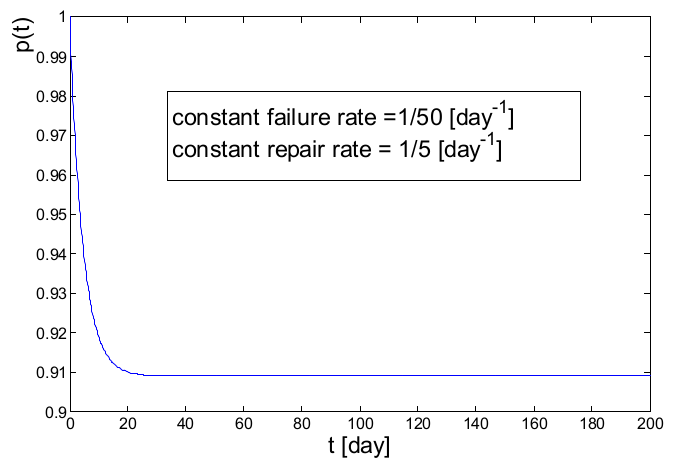
\includegraphics[width=0.7\textwidth]{example_6_1}
    \caption{Instantaneous availability}
\end{figure}

\section{Unrevealed failure}
\subsection{Safety Systems}
\paragraph*{An example} Risk: ignition of the gases in the oil tank, lightning strike or generation of
sparks due to electrostatic charges $\to$ Fire protection (see Fig.~\ref{fig:oil_tank}).
\begin{figure}[!htp]
    \centering
    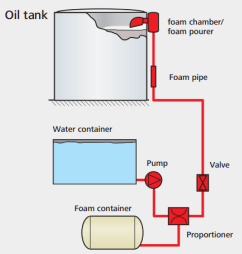
\includegraphics[width=.4\textwidth]{oil_tank}
    \caption{Oil tank}
    \label{fig:oil_tank}
\end{figure}

Safety systems are generally in standby until an accident occurs, which calls
for their operation. Hence, their \emph{components must be periodically tested}.
The components are unattended between tests and their failure is revealed only
when tested.

\subsection{Exercise: instantaneous availability of an unattanded component}
Find the instantaneous unavailability of an unattended component (no repair is
allowed) whose cumulative failure time distribution is $F(t)$.

\subsubsection*{Solution}
The istantaneous unavailability, i.e. the probability $q(t)$ that at time $t$
the component is not functioning is equal to the probability that it fails
before $t$
\begin{equation*}
    q(t) \equiv F(t)
\end{equation*}
\begin{equation*}
    q(t) = P\{X(t) = 0\} = P\{T\le t\} = F_T(t)
\end{equation*}

\subsection{Availability of a component under periodic test and maintenance}
The instantaneous availability is a periodic function of time (the interval
between two consecutive test is $T_p$). See Fig.~\ref{fig:instantaneous_avail}.

\begin{figure}[!htp]
    \centering
    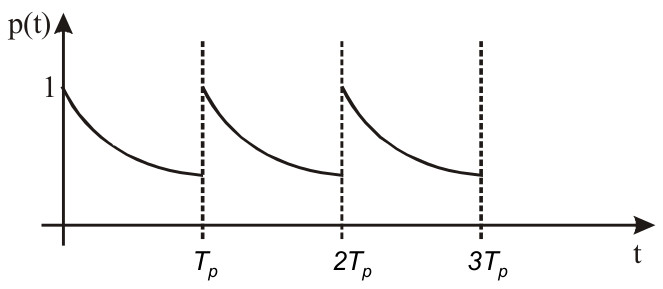
\includegraphics[width=.6\textwidth]{instantaneous_avail}
    \caption{Instantaneous availability is periodic}
    \label{fig:instantaneous_avail}
\end{figure}

The performance indicator used is the average unavailability over a period of
time $T_p$:
\begin{equation*}
    q_{T_p} = \frac{\int_0^{T_p}q(t)dt}{T_p} = \frac{\overline{\text{DOWNtime}}}{T_p}
\end{equation*}
where
\begin{itemize}
    \item $T_p$ is the complete maintenance cycle
    \item $\overline{\text{DOWNtime}}$ is the average time the system is not working
\end{itemize}

\subsection{Ideal case: instantaneous testing and maintenance}
Let's now assume that:
\begin{itemize}
    \item unavailability is due to unrevealed random failures (constant failure
    rate $\lambda$)
    \item \emph{instantaneous} and perfect testing and maintenance procedures
    are performed every $T_p$ hours
\end{itemize}

The instantaneous availability within a period $T_p$ coincides with the
reliability (Fig.~\ref{fig:instantaneous_avail}).

The average unavailability and availability are then:
\begin{equation*}
    q_{T_p} = \frac{\int_0^{T_p}q(t)dt}{T_p}  = \frac{\int_0^{T_p}F_T(t)dt}{T_p}
\end{equation*}
\begin{equation*}
    p_{T_p} = \frac{\int_0^{T_p}p(t)dt}{T_p}  = \frac{\int_0^{T_p}R(t)dt}{T_p} = 1-q_{T_p}
\end{equation*}

For different systems, we can compute $q_{T_p}$ and $p_{T_p}$ by first computing
their failure probability distribution $F_T(t)$ and reliability $R(t)$ and then
applying the above expressions.

For a system with constant failure rate $\lambda$ (good approximation only when
$\lambda t < 0.1$):
\begin{equation*}
    q_{T_p} = \frac{\int_0^{T_p}q(t)dt}{T_p}  = \frac{\int_0^{T_p}F_T(t)dt}{T_p} = \frac{\int_0^{T_p}(1-e^{-\lambda t})dt}{T_p} \approx \frac{\int_0^{T_p}\lambda t\,dt}{T_p} = \frac{\lambda T_p^2}{2T_p} = \frac{1}{2}\lambda T_p
\end{equation*}
\begin{equation*}
    p_{T_p} = 1-q_{T_p} = 1-\frac{1}{2}\lambda T_p
\end{equation*}

\subsection{A more realistic case: test and maintenance time is finite}
Let's assume that:
\begin{itemize}
    \item the test is performed after a time $\tau$ from the end of the previous test
    \item the test time $\tau_R$ is \emph{finite}
    \item unavailability is due to unrevealed random failures (constant failure rate $\lambda$)
\end{itemize}

We're asked to:
\begin{itemize}
    \item Draw the qualitative time evolution of the instantaneous availability
    \item Estimate the average unavailability and availability over the complete
    maintenance cycle period $T_p = \tau + \tau_R$.
\end{itemize}

\begin{figure}[!htp]
    \centering
    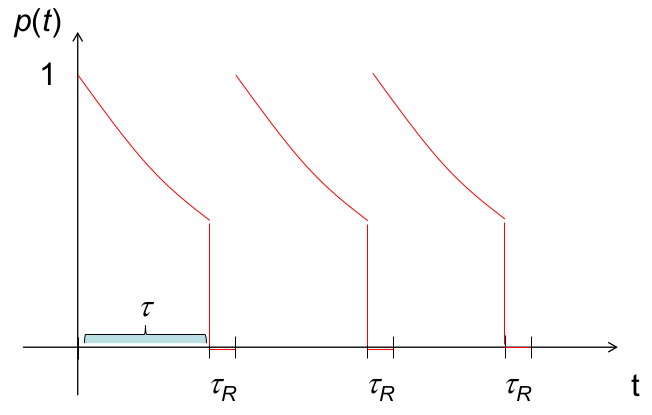
\includegraphics[width=.6\textwidth]{qualitative_inst_avail}
    \caption{Qualitative time evolution of the instantaneous availability}
\end{figure}

Assuming a finite repair time $\tau_R$ , this must be counted as DOWNtime, if
significant. Hence, the average unavailability and availability over the
complete maintenance cycle period $\tau+\tau_R$ will change into:
\begin{equation*}
    \overline{q} = \frac{\tau_R + \int_0^\tau F_T(t)dt}{\tau+\tau_R}
\end{equation*}
\begin{equation*}
    \overline{p} = \frac{\int_0^\tau R(t)dt}{\tau+\tau_R}
\end{equation*}

If the repair time $\tau_R$ is small compared with the period $\tau$ , we get:
\begin{equation*}
    \overline{q} = \frac{\tau_R + \int_0^\tau F_T(t)dt}{\tau}
\end{equation*}
\begin{equation*}
    \overline{p} = \frac{\int_0^\tau R(t)dt}{\tau}
\end{equation*}

\subsection{Single component under periodic maintenance}
\subsubsection*{Hypothesis}
\begin{itemize}
    \item The safety system is initially working: $q(0) = 0$ ; $p(0) = 1$;
    \item $\tau$ time interval between two consecutive maintenance interventions;
    \item $\tau_r$ duration of the maintenance intervention;
    \item Failure causes:
    \begin{itemize}
        \item random failure at any time $T \sim F_T(t)$;
        \item on-line switching failure on demand $\sim Q_0$;
        \item maintenance disables the component $\sim \gamma_0$ (human error during inspection, testing or repair).
    \end{itemize}
\end{itemize}

\subsubsection*{Objective}
Computation of the average unavailability over the lifetime $[0,T_M]$:
\begin{equation*}
    q_{[0,T_M]} = \frac{\overline{\text{DOWNtime}}}{T_M}
\end{equation*}

\subsubsection*{Method}
In order to compute the component average unavailability $\overline{q_{0T}}$ ,
we refer to its timeline (Fig.~\ref{fig:periodic_maintenance_timeline}).

\begin{figure}[!htp]
    \centering
    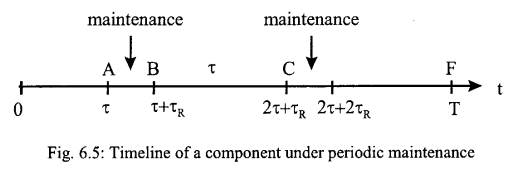
\includegraphics[width=.6\textwidth]{periodic_maintenance_timeline}
    \caption{Timeline}
    \label{fig:periodic_maintenance_timeline}
\end{figure}

\begin{equation*}
    \begin{split}
        q_{[0,T_M]} &= \frac{\int_0^{T_M}q(t)dt}{T_M} = \frac{\int_0^Aq(t)dt + \int_A^{T_M}q(t)dt}{T_M} \\
        &= \frac{\int_0^Aq(t)dt + k\left[\int_A^Bq(t)dt+\int_B^Cq(t)dt\right]}{T_M} \\
        &= \frac{\overline{\text{DOWNtime}_{0A}}+K[\overline{\text{DOWNtime}_{AB}}+ \overline{\text{DOWNtime}_{BC}}]}{T_M}  \\
        &= \frac{\overline{\text{DOWNtime}_{0T_M}}}{T_M} 
    \end{split}
\end{equation*}
where
\begin{equation*}
    k = \frac{T-\tau}{\tau+\tau_r}
\end{equation*}

\framebox[1.1\width]{Period from 0 to A} \par
Possible failure causes:
\begin{itemize}
    \item random failure ($E_1$);
    \item on-line switching failure on demand ($E_2$).
\end{itemize}

\begin{equation*}
    \forall t \in [0,A] \quad q_{0A}(t) = P(E_1)+P(E_2) - P(E_1\cap E_2) = F(t)+Q_0-F(t)Q_0
\end{equation*}

\begin{equation*}
    \begin{split}
        \overline{\text{DOWNtime}_{0A}} &= \int_0^\tau q_{0A}(t)dt \\
        &= \int_0^\tau [Q_0+(1-Q_0)F_T(t)]dt \\
        &= Q_0\tau + (1-Q_0)\int_0^\tau F_T(t)dt
    \end{split}
\end{equation*}

\framebox[1.1\width]{Period from A to B} \par
System under maintenance!
\begin{equation*}
    \forall t \in [A,B] \quad q_{AB}(t) = 1
\end{equation*}

\begin{equation*}
    \begin{split}
        \overline{\text{DOWNtime}_{AB}} &= \int_A^B q_{AB}(t)dt \\
        &= \int_\tau^{\tau_r} 1dt \\
        &= \tau_r
    \end{split}
\end{equation*}

\framebox[1.1\width]{Period from B to C} \par
Possible failure causes:
\begin{itemize}
    \item random failure ($E_1$);
    \item on-line switching failure on demand ($E_2$);
    \item maintenance disables the component ($E_3$)
\end{itemize}

\begin{equation*}
    \begin{split}
        \forall t \in [B,C] \quad q_{BC}(t) &= P(E_1)+P(E_2) +P(E_3) - P(E_1\cap E_2) - P(E_2\cap E_3) \\
        &\quad - P(E_1\cap E_3) + P(E_1\cap E_2\cap E_3) \\
        &= \gamma_0 + (1-\gamma_0)(Q_0 + (1-Q_0)F(t))
    \end{split}
\end{equation*}

\begin{equation*}
    \begin{split}
        \overline{\text{DOWNtime}_{BC}} &= \int_0^\tau q_{BC}(t)dt \\
        &= \gamma_0\tau + (1-\gamma_0)\left[Q_0\tau + (1-Q_0)\int_0^\tau F_T(t)dt\right]
    \end{split}
\end{equation*}

\begin{equation*}
    \begin{split}
        \overline{\text{DOWNtime}_{0T_M}} &= Q_0\tau + (1-Q_0)\int_0^\tau F_T(t)dt\,+\\
        &\quad + \frac{T-\tau}{\tau+\tau_r} \left\{\tau_R + \gamma_0\tau + (1-\gamma_0)\left[Q_0\tau + (1-Q_0)\int_0^\tau F_T(t)dt\right] \right\}
    \end{split}
\end{equation*}

\begin{equation*}
    \begin{split}
        q_{[0,T_M]} &= \frac{\overline{\text{DOWNtime}_{0T_M}}}{T_M} \\
       &= \frac{Q_0\tau}{T_M} + \frac{1-Q_0}{T_M}\int_0^\tau F_T(t)dt\,+\\
       &\quad + \frac{1}{\tau+\tau_r} \left\{\tau_R + \gamma_0\tau + (1-\gamma_0)\left[Q_0\tau + (1-Q_0)\int_0^\tau F_T(t)dt\right] \right\}
    \end{split}
\end{equation*}
          
We simplify under the following assumptions:
\begin{itemize}
    \item $\tau\ll T_M$
    \item $\int_0^\tau F_T(t)dt \le \tau$
    \item $\tau_R \ll \tau$
\end{itemize}

\begin{equation*}
    \begin{split}
        q_{[0,T_M]} &= \frac{\overline{\text{DOWNtime}_{0T_M}}}{T_M} \\
       &= \xcancel{\frac{Q_0\tau}{T_M}} + \xcancel{\frac{1-Q_0}{T_M}\int_0^\tau F_T(t)dt}\,+\\
       &\quad + \frac{1}{\tau+\xcancel{\tau_r}} \left\{\tau_R + \gamma_0\tau + (1-\gamma_0)\left[Q_0\tau + (1-Q_0)\int_0^\tau F_T(t)dt\right] \right\} \\
       &= \frac{\tau_R}{\tau} + \gamma_0 + (1-\gamma_0)\left[Q_0 + \frac{1-Q_0}{\tau}\int_0^\tau F_T(t)dt\right]
       \end{split}
\end{equation*}

Often in practice, $\gamma_0 \ll 1$ , $Q_0 \ll 1$. Then:
\begin{equation*}
    q_{[0,T_M]} \cong \frac{\tau_R}{\tau} + \gamma_0 + (1-\xcancel{\gamma_0})\left[Q_0 + \frac{1-\xcancel{Q_0}}{\tau}\int_0^\tau F_T(t)dt\right]
\end{equation*}

We now consider an exponential system with small, constant failure rate:
\begin{equation*}
    \lambda \implies F_T(t) = 1 - e^{-\lambda t} \cong \lambda \cdot t
\end{equation*}

The average unavailability reads:
\begin{equation*}
    q_{[0,T_M]} \cong \frac{\tau_R}{\tau} + \gamma_0 + Q_0 + \frac{1}{2}\lambda\tau
\end{equation*}

From this formula it is possible to distinguish each contribution to the
unavailability of the component, as in Table~\ref{tab:periodic_maintenance_components}

\begin{table}[!htp]
    \centering
    \begin{tabular}{ll}
        \toprule
        Term & Cause \\
        \midrule
        
        $\frac{\tau_R}{\tau}$ & unavailability during maintenance \\[2ex]
        $\gamma_0$ & unavailability due to an error which leaves the unit DOWN after test \\[2ex]
        $Q_0$ & unavailability due to the switch failing on demand \\[2ex]
        $\frac{1}{2}\lambda\tau$ & unavailability due to random, unrevealed failures between successive tests \\
        \bottomrule
    \end{tabular}
    \caption{Terms of $q_{[0,T_M]}$ vs. the respective causes}
    \label{tab:periodic_maintenance_components}
\end{table}

\section{Where to study?}
\paragraph*{\color{BrickRed}Red book}
\begin{itemize}
    \item Chapter 6
\end{itemize}

\paragraph*{\color{PineGreen}Green book}
\begin{itemize}
    \item All problems in Chapter 6
\end{itemize}